\documentclass[10pt,letter]{article}
\usepackage[utf8]{inputenc}
\usepackage{amsmath}
\usepackage{amsfonts}
\usepackage{amssymb}
\usepackage{graphicx}
\usepackage[margin=1in]{geometry}


\begin{document}

\begin{titlepage}
\title{PHYS 5794 Homework 6}
\date{March 14, 2016}
\author{Thomas Edwards}
\maketitle
\end{titlepage}

\section{Problem 1}

\subsection{Problem Statement}

Write a program to solve a driven pendulum problem that we discussed in the class. Suppose that
a pendulum consists of a light string of length $l$ and a point mass m attached to the end of the
rod. The end of the string is tied to a heavy horizontal bar aligned along with the x axis and attached
to a heavier stand. The pendulum swings in the $yz$ plane. Three kinds of forces are acting
on the pendulum: gravity, frictional force linearly proportional to the angular velocity $-kld\theta/dt$,
and driving force $f_d^0\cos(w_0t)$, where $k$ is a proportional constant, $f_d^0$ is the amplitude, and $w_0$ is the
angular frequency of the driving force. Initially the pendulum is located vertically $(\theta = 0)$, where $\theta$
is the angle between the rod and the vertical line. You may choose the range of the angle as $(-\pi,
\pi)$ or $(0, 2\pi)$. The initial angular velocity of the pendulum is $d\theta/dt = \omega = 11.431 sec^{-1}$. Use the
following numbers for the parameters: $l=30$ cm, $(k/m)\sqrt{l/g} = 0.5$, $w_0\sqrt{l/g}=2/3$,$\tau=3\pi/100$ (time
interval), and $t = 1000 \times \tau$ (elapsed time). To solve this differential equation, a dimensionless form
is recommended. (20 pts)
The following issues should be addressed either in your report. The axes of any plots must be properly
labeled.

(i) Write the initial conditions in dimensionless units. You may use $\sqrt{l/g}$ as the time unit.

(ii) Solve the 2nd-order differential equation by using the fourth-order Runge-Kutta method
when$f_d^0= 0$. Plot the angular velocity $w(t)$ vs the angle $\theta(t)$ as time evolves ($t = 1000 \times \tau$).
Explain your numerical result.

(iii) Solve the 2nd-order differential equation by using the fourth-order Runge-Kutta method
when$f_d^0= 0.89mg$. Plot the angular velocity $w(t)$ vs the angle $\theta(t)$ as time evolves ($t = 1000 \times \tau$).
Explain your numerical result.

(iv) Solve the 2nd-order differential equation by using the fourth-order Runge-Kutta method
when$f_d^0= 1.145mg$. Plot the angular velocity $w(t)$ vs the angle $\theta(t)$ as time evolves ($t = 1000 \times \tau$).
Does your numerical result make sense physically?

\subsection{Method}

To begin, we rewrite the differential equation in a form that has dimensionless units. We start with
\begin{align}
ml\frac{d^2\theta}{dt^2} &= -mg\sin\theta - kl \frac{d\theta}{dt} + f_d^0\cos{(w_0t)} \notag \\
\frac{d^2\theta}{dt^2} &= -\frac{g}{l}\sin\theta - \frac{k}{m} \frac{d\theta}{dt} + \frac{f_d^0}{ml}\cos{(w_0t)}.
\end{align}
Now, let $t=\sqrt{l/g}t'$ in order to make time dimensionless. Then
\begin{align}
\frac{d^2\theta}{dt'^2}\frac{g}{l} &= -\frac{g}{l}\sin\theta - \frac{k}{m} \sqrt{\frac{g}{l}}\frac{d\theta}{dt'} + \frac{f_d^0}{ml}\cos{\left(w_0\sqrt{\frac{l}{g}}t'\right)} \notag \\
\frac{d^2\theta}{dt'^2} &= -\sin\theta - \frac{k}{m} \sqrt{\frac{l}{g}}\frac{d\theta}{dt'} + \frac{f_d^0}{mg}\cos{\left(w_0\sqrt{\frac{l}{g}}t'\right)}.
\end{align}
Now, let $q=(k/m)\sqrt{l/g}$, $b= f_d^0/mg$, and $\bar{w_0} = w\sqrt{l/g}$. We now have
\begin{align}
\frac{d^2\theta}{dt'^2}&= -\sin\theta - q\frac{d\theta}{dt'} +b\cos{\bar{w_0}t'}.
\end{align}

We now allow $d\theta/dt = w$, which then allows us break up this second order differential equation in to two first order equations. This is then solved by the Runge-Kutta method in a fourth order scheme, where
\begin{align}
k_{\theta 1} &= w \notag\\
k_{\theta 2} &= w + \frac{h}{2}k_{\theta 1} \notag \\
k_{\theta 3} &= w + \frac{h}{2}k_{\theta 2} \notag \\
k_{\theta 4} &= w + hk_{\theta 3} \notag \\
\theta(t+h) &= \theta(t) + \frac{h}{6}(k_{\theta 1} + 2k_{\theta 2} + 2k_{\theta 3} +k_{\theta 1}) \notag \\
k_{w 1} &= f(t, \theta(t), w(t)) \notag \\
k_{w 2} &= f(t+ \frac{h}{2}, \theta(t)+ \frac{h}{2}k_{\theta 1}, w(t)+ \frac{h}{2}k_{w 1}) \notag \\
k_{w 3} &= f(t+ \frac{h}{2}, \theta(t)+ \frac{h}{2}k_{\theta 2}, w(t)+ \frac{h}{2}k_{w 2}) \notag \\
k_{w 4} &= f(t+ h, \theta(t)+ hk_{\theta 3}, w(t)+hk_{w3}) \notag \\
w(t+h) &= w(t) + \frac{h}{6}(k_{w 1} + 2k_{w 2} + 2k_{w 3} +k_{w 1}) \notag \\
t&=t+h \notag
\end{align}
where
\begin{align}
 f(t, \theta, w)  &= -\sin{\theta}-qw+n\cos{(\bar{w}_0t)}.
\end{align}


\subsection{Verification of Program}

This program was tested by attempting to solve the equation
\begin{align}
y'' &= -4\pi^2y
\end{align}
with initial conditions $y(0)=1$, $y'(0)=0$. The solution, both analytic and numeric, are shown in the plot below.
\begin{figure}[h]
  \centering
    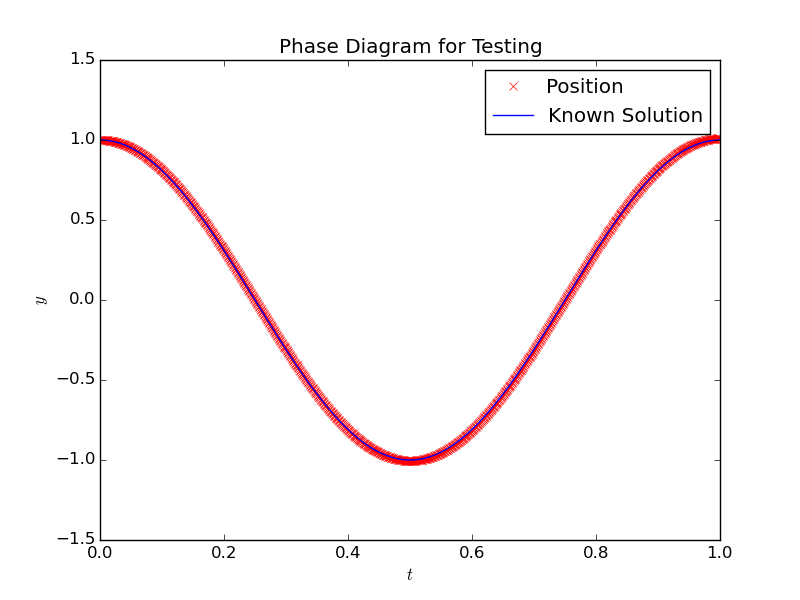
\includegraphics[width=.5\textwidth]{homework6_problem1_plot10}
  \caption{Phase diagram for verification procedure.}
\end{figure}
As we can see from the overlapping solutions, the solver appears to be working.

\pagebreak
\subsection{Data}

The three systems are solved and their phase diagrams plotted. They are below.
\begin{figure}[h]
  \centering
    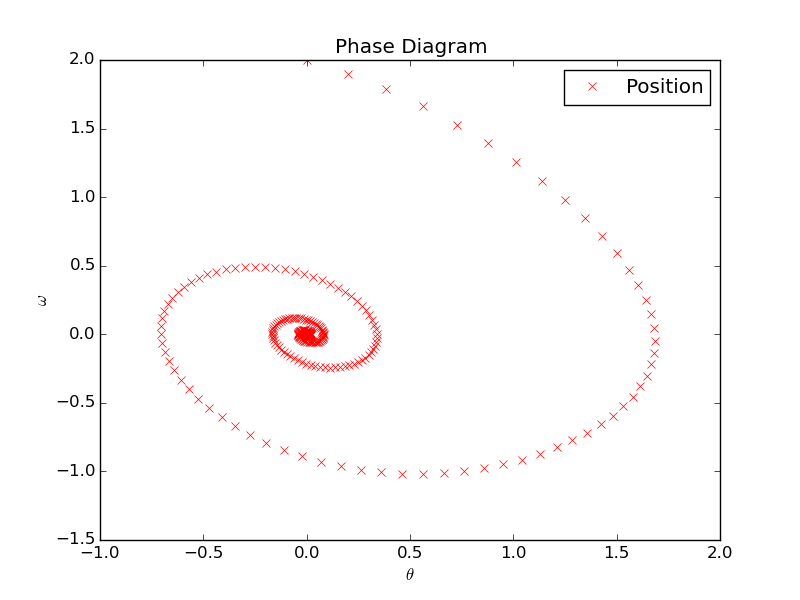
\includegraphics[width=.5\textwidth]{homework6_problem1_plot1}
  \caption{Phase diagram for $f_d^0 = 0$.}
\end{figure}

\begin{figure}[h]
  \centering
    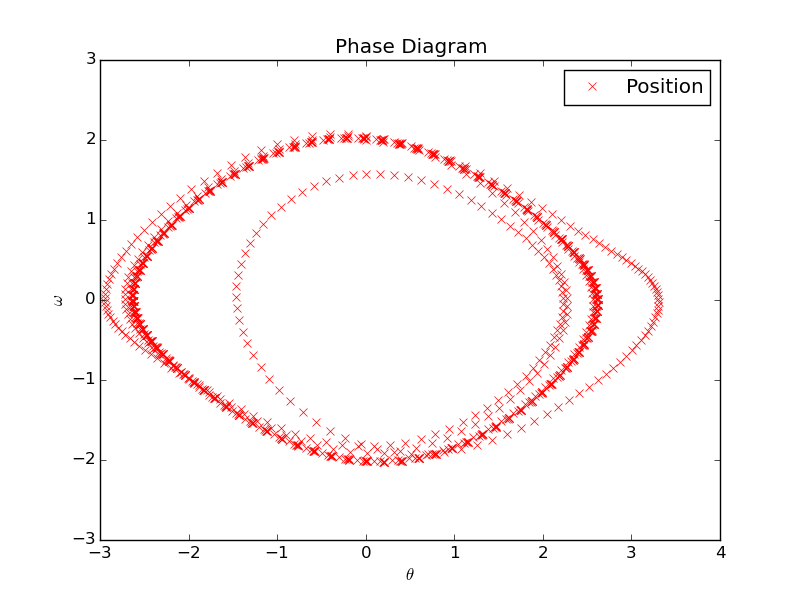
\includegraphics[width=.5\textwidth]{homework6_problem1_plot3}
  \caption{Phase diagram for $f_d^0 = 0.89mg$.}
\end{figure}

\begin{figure}[h]
  \centering
    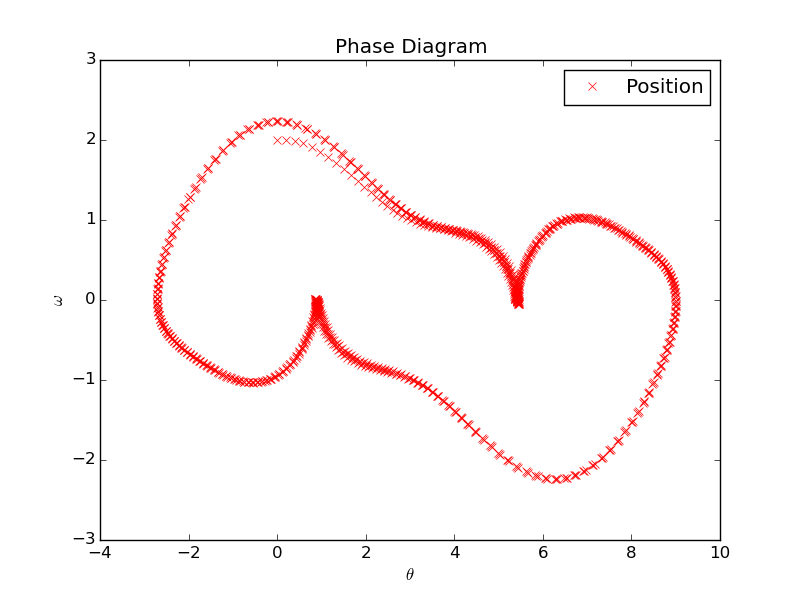
\includegraphics[width=.5\textwidth]{homework6_problem1_plot5}
  \caption{Phase diagram for $f_d^0 = 1.145mg$.}
\end{figure}

\pagebreak

\subsection{Analysis}
All three solutions appear to start correctly in their initial conditions, and then evolve until a steady state solution in found. In the case of the first system, that solution is certainly one where the pendulum ends at rest. In the other cases, however, the driving term is able to produce a steady state solution that is stable, and is held for the remaining period of the simulation time once the state has been found.

\subsection{Interpretation}

We see immediately that the first case, where the system is not driven, quickly spirals down to a solution where the pendulum is at rest. This is completely expected, and is a good suggestions that the solver is working correctly.

The second case shows a solution where the driving provides a steady state solution that appears to be the damped-driven harmonic oscillator, which is expected considering the amplitude of the driving force compared to that of the frictional term.

The third case is certainly the overdriven solution, considering it's phase diagram. It does make physical sense, especially taking in to account how high the amplitude of the driving term is compared to the rest of the forces.

\subsection{Log}

This problem took approximately 6 hours.

\section{Problem 2}

\subsection{Problem Statement}

Write programs to solve the following ordinary differential equation with two boundary conditions:
$$\frac{d^2y}{dx^2} = -4\pi^2y(x)$$
with $y(x=0) = 1$ and $dy/dx(x=1)=2\pi$.

(i) Solve the differential equation analytically.

(ii) What have you used for your initial guess, dy/dx(x = 0)?

(iii) Compare your numerical result with the analytical result (the answer to (i)).

(iv) Solve the same differential equation as above using the 4th-order Runge-Kutta method only
twice instead of using many times in the shooting method. Refer to the lecture notes right
after discussion on the shooting method. What have you used for the two arbitrary values of
the initial conditions?

\subsection{Method}

First, the analytic solution to the differential equation follows simply as a simple harmonic oscillator with the general solution
\begin{align}
y(x) = A\cos{wx} + B\sin{wx}.
\end{align}
Applying the boundary condition $y(x=0) = 1$ gives us 
\begin{align}
A\cos{0} + B\sin{0} &= 1 \notag \\
A &= 1
\end{align}
which then makes our solution have the form
\begin{align}
y(x) = \cos{wx} + B\sin{wx}.
\end{align}
Taking the derivative of this equation with respect to $x$ gives us
\begin{align}
\frac{dy}{dx} = -w\sin{wx} + wB\cos{wx}.
\end{align}
We then apply our boundary condition $dy/dx(x=1)=2\pi$ to get
\begin{align}
2\pi = w(-\sin{w} + B\cos{w}).
\end{align}
Solving for $B$ nets us
\begin{align}
\frac{\frac{2\pi}{w} + \sin{w}}{\cos{w}} =B.
\end{align}
Differentiating once more gives us
\begin{align}
\frac{d^2y}{dx^2} &= -w^2(\cos{wx} + B\sin{wx}) \notag \\
-w^2(\cos{wx} + B\sin{wx}) &= -4\pi^2y \notag \\
-w^2(\cos{wx} + B\sin{wx}) &= -4\pi^2(\cos{wx} + B\sin{wx}).
\end{align}
which shows quite clearly that $w = 2\pi$. Using this information to simplify $B$ gives\begin{align}
B&=\frac{\frac{2\pi}{2\pi} + \sin{2\pi}}{\cos{2\pi}} \notag \\
&= 1.
\end{align}
This then gives us a final solution of 
\begin{align}
y(x) = \cos{2\pi x} + \sin{2\pi x}.
\end{align}

The numerical solution of this problem follows a similar form to that of the first problem, except that there is a small variation in the methodology. Since we know a boundary condition of the system at $x=0$ and a condition for the derivative at $x=1$, we need to produce a solution using our known condition of $y(x=0)$ and compare that to the condition at $y'(x=1)$. To do this, we first choose some guess term $\delta$ and a small perturbation term $\epsilon$, which in this case have been chosen as $\delta = 0$ and $\epsilon = 0.001$.

First, however, we make a small clarification on notation. Let us assume that $y_1 = y$, $dy_1/dx = y_2$, and $dy_2/dx = -4\pi^2y_1$. This will allow us to separate the second order equation in to two first order equations, and further simplify the nomenclature.

We then use the fourth order Runge-Kutta solver to find a solution to our differential equation for $y_1$ given that $y_1(x=0)$ is known and assuming that $y_2(x=0) = \delta = \delta_0$. We then compare the solution at $y^{s1}_{2}(x=1)$ ($s1$ here used to signify a ``solution'' variable, as opposed to our known quantity) to our known boundary condition at $y_2(x=1)$, and save it as $f_0$.

Next, we repeat this process, except that we modify the initial $y_2$ slightly by letting $y_2(x=0) = \delta+\epsilon= \delta_1$. Again, we save the difference between the solution $y^{s2}_2$ to the known condition, this time as $f_1$.

From here we compare the differences of the previous two steps $\Delta = f_1 - f_0$, and compare them to a tolerance value, which in this case was set to be $10^{-15}$ by default. If the magnitude of the comparison is below our tolerance value, we assume we have found the solution.

If the comparison is not below our tolerance value, however, we simply adjust our guess by the secant method, letting
\begin{align}
\delta_2 &= \delta_1 - \frac{\delta_1-\delta_0}{\Delta}f_1 \\
\delta_0 &= \delta_1 \\
\delta_1 &= \delta 2.
\end{align}
We then restart the process with a new set of guesses, and proceed until we either find a solution or a set maximum number of iterations has been run.




\subsection{Verification of Program}

This solution found by this program was compared to the analytic solution, and is shown in the Data section.
\subsection{Data}

The data for this problem comes in the form of two plots, which are shown below.

\begin{figure}[h]
  \centering
    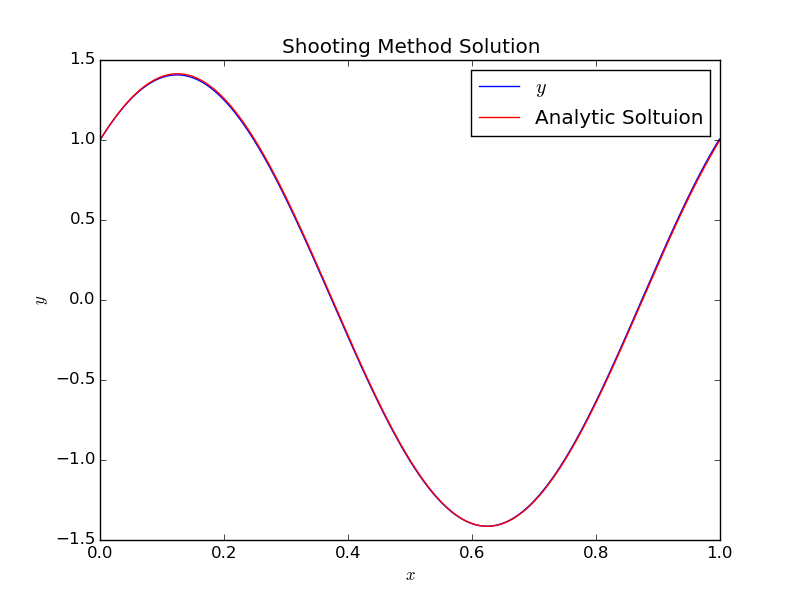
\includegraphics[width=.7\textwidth]{homework6_problem2_plot1}
  \caption{Solution using the shotting method (in blue) and a comparison to the analytic solution (in red).}
\end{figure}
\begin{figure}[h]
  \centering
    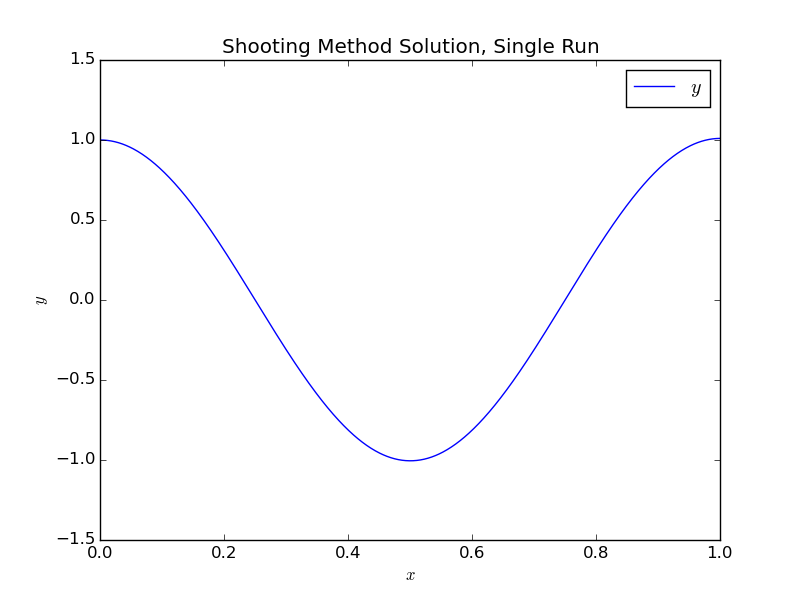
\includegraphics[width=.7\textwidth]{homework6_problem2_plot2}
  \caption{Solution only using a single run of Runge-Kutta.}
\end{figure}

\subsection{Analysis}

It is clear by the comparison between the red and blue (mostly overlapping) lines that the solution is very close to the analytic solution, and that the program is running correctly. This program converged to a solution in only 4 iterations as well, which is surprisingly fast.

It is also clear that just using a fourth order Runge-Kutta solver was not sufficient, as only using a single iteration of the Runge-Kutta gave a solution that was not correct, and was instead not bound by the secondary boundary condition.
\subsection{Interpretation}

The results are as expected, which is primarily due to the corrections enforced by the second boundary condition. As mentioned in the last section, without that condition the solution simply doesn't converge to the correct solution, even though it is technically \emph{a} solution to the equation, albeit the incorrect one.
 
\subsection{Log}

This problem took approximately 6 hours.

\end{document}